%% FullCourse_10Lecs -- Lecture 7, Act 5 (MEASURE, part 1/2): Limits of LLMs
%% ch14 rebuild (2026-07-07), per Lec07_ch14_Rebuild_Plan_2026-07-07.md.
%% Reused frames copied verbatim (with renumbered cross-references) from
%%   archive_pre_split/pre_ch14_rebuild_2026-07-07/Lec07_T3b_Limits_Measurement.tex
%%   (limits section + Brain Metaphor; the AI-exposure/YVP instrument arc moves to T5b)
%% Reframed to chapter14 sec. 14.6.1's "five structural limits", each traced
%% architectural root -> research implication; YVP capstone verified against
%% NBER WP 35110 (headline figures corroborated 2026-07-07).

%% Shared preamble for the FullCourse_10Lecs topic decks.
%%
%% Each topic .tex \input's this file, then defines its own \title, \date
%% override (if any), \graphicspath, and \begin{document}.
%%
%% Reconstructed verbatim from the inlined copy preserved in
%% Lec10_Case_Studies/Lec10_T8_Case6_DeepRamsey.tex (lines 23-190), which is
%% explicitly annotated there as "from ../shared_preamble.tex, copied verbatim".
%% Base preamble matches MiniCourse_8hr/Slides/shared_preamble.tex; this version
%% additionally provides \sectiondivider, the conceptbox/cautionbox/examplebox/
%% takeawaybox tcolorboxes, and \compacttables used across the split decks.

\documentclass[10pt,english,aspectratio=169]{beamer}

\usepackage{ae,aecompl}
\usepackage[T1]{fontenc}
\usepackage{textcomp}
\usepackage[utf8]{inputenc}
\usepackage{babel}
\usepackage{datetime2}

\setcounter{secnumdepth}{3}
\setcounter{tocdepth}{3}

\usepackage{amsmath, amssymb, amsthm, graphicx}
\usepackage{booktabs, multirow}
\usepackage{tikz}
\usepackage{pgfplots}
\pgfplotsset{compat=1.16}
\usepackage[most]{tcolorbox}
\tcbuselibrary{skins, breakable, theorems}
\usepackage{listings}
\usepackage{xcolor}

\lstset{
  basicstyle=\ttfamily\small,
  keywordstyle=\color{blue!80!black}\bfseries,
  commentstyle=\color{green!50!black}\itshape,
  stringstyle=\color{orange!80!black},
  backgroundcolor=\color{gray!8},
  frame=single,
  rulecolor=\color{gray!40},
  breaklines=true,
  showstringspaces=false,
  numbers=none,
}

\lstdefinestyle{pythonstyle}{
    language=Python,
    basicstyle=\ttfamily\footnotesize,
    keywordstyle=\color{blue!80!black}\bfseries,
    commentstyle=\color{green!50!black}\itshape,
    stringstyle=\color{orange!80!black},
    frame=single,
    breaklines=true,
    showstringspaces=false,
    numbers=left,
    numbersep=5pt,
    numberstyle=\tiny\color{gray},
    backgroundcolor=\color{gray!8},
    rulecolor=\color{gray!40}
}

\ifx\hypersetup\undefined
  \AtBeginDocument{%
    \hypersetup{bookmarks=false,breaklinks=true,pdfborder={0 0 0},colorlinks=true,
      linkcolor=DarkText,urlcolor=RedTitle}%
  }
\else
  \hypersetup{bookmarks=false,breaklinks=true,pdfborder={0 0 0},colorlinks=true,
    linkcolor=DarkText,urlcolor=RedTitle}%
\fi

\makeatletter
\newcommand\makebeamertitle{%
  \begin{frame}[plain]
    \vspace*{1.0cm}
    \centering
    {\usebeamerfont{title}\usebeamercolor[fg]{title}\inserttitle\par}
    \vspace{1.0cm}
    {\usebeamerfont{author}\usebeamercolor[fg]{author}\insertauthor\par}
    \vspace{0.2cm}
    {\usebeamerfont{date}\usebeamercolor[fg]{date}\insertdate\par}
  \end{frame}}%
\AtBeginDocument{%
  \let\origtableofcontents=\tableofcontents
  \def\tableofcontents{\@ifnextchar[{\origtableofcontents}{\gobbletableofcontents}}
  \def\gobbletableofcontents#1{\origtableofcontents}%
}

\usetheme{metropolis}
\usefonttheme{professionalfonts}

\definecolor{LightGray}{RGB}{230,230,230}
\definecolor{RedTitle}{RGB}{0,0,200}
\definecolor{VeryLightGray}{RGB}{245,245,245}
\definecolor{DarkText}{RGB}{0,0,0}

\setbeamercolor{background canvas}{bg=white}
\setbeamercolor{title}{fg=RedTitle}
\setbeamercolor{author}{fg=DarkText}
\setbeamercolor{date}{fg=DarkText}
\setbeamercolor{frametitle}{bg=VeryLightGray,fg=DarkText}
\setbeamercolor{normal text}{fg=DarkText}
\setbeamerfont{title}{size=\large}

\setbeamersize{text margin left=5mm, text margin right=5mm}
\addtobeamertemplate{frametitle}{}{\vspace{-0.5em}}
\newcommand{\reducevspace}{\vspace{-0.5cm}}

% Shared section divider and box styles for split topic decks.
\newcommand{\sectiondivider}[2]{%
\begin{frame}[plain,noframenumbering]
\begin{center}
\vfill
{\Large\textbf{#1}\par}
\vspace{0.35cm}
{\normalsize #2\par}
\vfill
\end{center}
\end{frame}
}

\newtcolorbox{conceptbox}[1][]{
  colback=blue!3,
  colframe=RedTitle!55,
  boxrule=0.35mm,
  arc=1mm,
  left=2mm,
  right=2mm,
  top=1mm,
  bottom=1mm,
  #1
}
\newtcolorbox{cautionbox}[1][]{
  colback=red!3,
  colframe=red!50!black,
  boxrule=0.35mm,
  arc=1mm,
  left=2mm,
  right=2mm,
  top=1mm,
  bottom=1mm,
  #1
}
\newtcolorbox{examplebox}[1][]{
  colback=green!3,
  colframe=green!45!black,
  boxrule=0.35mm,
  arc=1mm,
  left=2mm,
  right=2mm,
  top=1mm,
  bottom=1mm,
  #1
}
\newtcolorbox{takeawaybox}[1][]{
  colback=VeryLightGray,
  colframe=RedTitle!55,
  boxrule=0.35mm,
  arc=1mm,
  left=2mm,
  right=2mm,
  top=1mm,
  bottom=1mm,
  #1
}
\newcommand{\compacttables}{\renewcommand{\arraystretch}{1.15}}

\setbeamertemplate{navigation symbols}{}
\setbeamertemplate{footline}{%
  \hfill%
  \usebeamercolor[fg]{page number in head/foot}%
  \usebeamerfont{page number in head/foot}%
  \insertframenumber\,/\,\inserttotalframenumber\kern1em\vskip2pt%
}

\makeatother

\author{Zhigang Feng}
% "date with time": compile timestamp so each build is identifiable.
\date{\today\ \DTMcurrenttime}


\metroset{sectionpage=none}

\graphicspath{{./pic/}{../../MiniCourse_8hr/Slides/Module3_LLM_Text/pic/}{../}}

\usetikzlibrary{arrows.meta, positioning, shapes.geometric, fit, backgrounds}

%% Lec07 shared MAP slide: "one map, five acts" recurring diagram.
%% Adapted from ../Lec09_Agentic_AI/lec09_map.tex (\LecNineMap -> \LecSevenMap).
%% Input this file AFTER ../shared_preamble.tex (needs RedTitle, VeryLightGray)
%% and call \LecSevenMap{k} inside a frame, where k in {1..5} highlights the
%% current act ("you are here") and k = 0 renders the closing reprise with all
%% five acts complete (used by T5b's closing frame).
%% Filename deliberately does not match the build glob Lec*_T*.tex, so the
%% build script never tries to compile it standalone.

\newcommand{\LecSevenMap}[1]{%
% Precompute per-box style selectors; TikZ option lists are comma-split before
% TeX conditionals run, so \ifnum must not sit inside a [...] options list.
\ifnum#1=0
  \tikzset{lecmapa/.style={lecmapdone}, lecmapb/.style={lecmapdone},
           lecmapc/.style={lecmapdone}, lecmapd/.style={lecmapdone},
           lecmape/.style={lecmapdone}}%
\else
  \tikzset{lecmapa/.style={}, lecmapb/.style={}, lecmapc/.style={},
           lecmapd/.style={}, lecmape/.style={}}%
  \ifnum#1=1 \tikzset{lecmapa/.style={lecmapcur}}\fi
  \ifnum#1=2 \tikzset{lecmapb/.style={lecmapcur}}\fi
  \ifnum#1=3 \tikzset{lecmapc/.style={lecmapcur}}\fi
  \ifnum#1=4 \tikzset{lecmapd/.style={lecmapcur}}\fi
  \ifnum#1=5 \tikzset{lecmape/.style={lecmapcur}}\fi
\fi
\begin{center}
\begin{tikzpicture}[
    act/.style={rectangle, rounded corners, draw=black!60, fill=VeryLightGray,
        minimum width=2.6cm, minimum height=0.92cm, text width=2.5cm,
        align=center, font=\scriptsize, text=DarkText},
    lecmapcur/.style={draw=RedTitle, very thick, fill=orange!20},
    lecmapdone/.style={draw=green!45!black, thick, fill=green!10},
    q/.style={font=\tiny\itshape, text width=2.7cm, align=center, text=black!70},
    sat/.style={rectangle, rounded corners, draw=black!45, dashed, fill=white,
        text width=5.0cm, align=center, font=\tiny, text=black!70,
        minimum height=0.5cm},
    barlab/.style={font=\tiny\bfseries, text=black!60},
    arr/.style={-{Stealth[length=2mm]}, thick, gray!60}
]
    % --- five act boxes ---
    \node[act, lecmapa] (a1) at (0,0)
        {\textbf{7.1 FRAME}\\ \tiny text as measurement};
    \node[act, lecmapb] (a2) at (2.85,0)
        {\textbf{7.2 REPRESENT}\\ \tiny tokens $\to$ vectors};
    \node[act, lecmapc] (a3) at (5.7,0)
        {\textbf{7.3 ATTEND}\\ \tiny attention \& Transformer};
    \node[act, lecmapd] (a4) at (8.55,0)
        {\textbf{7.4 PRETRAIN}\\ \tiny LMs \& alignment};
    \node[act, lecmape] (a5) at (11.4,0)
        {\textbf{7.5 MEASURE}\\ \tiny limits, apps, validation};
    \draw[arr] (a1) -- (a2);
    \draw[arr] (a2) -- (a3);
    \draw[arr] (a3) -- (a4);
    \draw[arr] (a4) -- (a5);
    % --- the student question each act answers ---
    \node[q] at (0,-0.82)    {what generates\\ this text?};
    \node[q] at (2.85,-0.82) {how do we turn it\\ into numbers?};
    \node[q] at (5.7,-0.82)  {how does context\\ get encoded?};
    \node[q] at (8.55,-0.82) {where does a pretrained\\ model come from?};
    \node[q] at (11.4,-0.82) {is my measure valid ---\\ and defensible?};
    % --- "you are here" marker above the current act ---
    \ifnum#1=1 \node[font=\scriptsize\bfseries, text=RedTitle] at (0,0.95)
        {you are here\ $\blacktriangledown$};\fi
    \ifnum#1=2 \node[font=\scriptsize\bfseries, text=RedTitle] at (2.85,0.95)
        {you are here\ $\blacktriangledown$};\fi
    \ifnum#1=3 \node[font=\scriptsize\bfseries, text=RedTitle] at (5.7,0.95)
        {you are here\ $\blacktriangledown$};\fi
    \ifnum#1=4 \node[font=\scriptsize\bfseries, text=RedTitle] at (8.55,0.95)
        {you are here\ $\blacktriangledown$};\fi
    \ifnum#1=5 \node[font=\scriptsize\bfseries, text=RedTitle] at (11.4,0.95)
        {you are here\ $\blacktriangledown$};\fi
    \ifnum#1=0 \node[font=\scriptsize\bfseries, text=green!45!black] at (5.7,0.95)
        {all five acts complete};\fi
    % --- bottom band: the measurement sandwich ---
    \fill[blue!10]   (-1.3,-1.55) rectangle (1.40,-1.22);
    \fill[green!10]  (1.65,-1.55) rectangle (9.85,-1.22);
    \fill[orange!15] (10.1,-1.55) rectangle (12.7,-1.22);
    \node[barlab] at (0.05,-1.385) {WHY TEXT = MEASUREMENT};
    \node[barlab] at (5.75,-1.385) {HOW THE MACHINE READS TEXT};
    \node[barlab] at (11.4,-1.385) {MEASURE, VALIDATE, DISCLOSE};
    % --- the recurring spine (text DGP), printed under the band ---
    \node[font=\tiny\itshape, text=black!60] at (5.7,-1.83)
        {the spine:\ \ $x_i = g(s_i,\,a_i,\,c_i)+\varepsilon_i
         \;\longrightarrow\; m(x_i)
         \;\longrightarrow\; y_i = \beta\,m(x_i)+\gamma z_i+u_i$};
    % --- dashed satellites: the neighbouring lectures ---
    \node[sat] at (2.0,-2.42)
        {\textit{before 7.1:} Lec03--04 gave you neural nets, backprop \& PyTorch --- Lec07 teaches them to read};
    \node[sat] at (9.8,-2.42)
        {\textit{after 7.5:} Lec08 RAG (grounded memory) $\to$ Lec09 agents (grounded action) $\to$ Lec10 cases};
\end{tikzpicture}
\end{center}
}


\title[AI for Econ Research]{AI for Economic Research: Dynamic Models, Language, and Agents\\
Lecture 7.5a: Limits of LLMs}

\begin{document}

\makebeamertitle

%=============================================================================
\begin{frame}{Lecture 7 in One Map}
\LecSevenMap{5}
\medskip
\textit{\footnotesize Route: five structural limits, each traced from its architectural root to its research implication (part 1/2 of MEASURE --- what breaks); part 2/2 covers what works, and how to defend it.}
\end{frame}

%=============================================================================
\section{Five Structural Limits}
\sectiondivider{Five Structural Limits}{Architecture in, research implication out}

\begin{frame}{Five Limits, Five Architectural Roots}
\textbf{None of these are bugs awaiting a patch --- each follows from how the machine is built.}
\begin{center}
\renewcommand{\arraystretch}{1.35}
\footnotesize
\begin{tabular}{p{3.0cm} p{4.3cm} p{4.9cm}}
\toprule
\textbf{Limit} & \textbf{Architectural root} & \textbf{Research implication} \\
\midrule
1. Knowledge cutoff & knowledge frozen in weights; updating $=$ retraining & provide the sources in the prompt; never assume ``it knows the event'' \\
2. Hallucination & max-likelihood over \emph{form}, not truth & every citation and number is a draft until independently verified \\
3. Context window & attention cost $O(n^2)$ & chunking severs cross-references; full filings may not fit \\
4. Lost in the middle & positional attention bias (U-curve) & extraction accuracy depends on \emph{where} the passage sits --- non-classical error \\
5. Prompt sensitivity \& primacy & ICL: the prompt is the prior & freeze, version, and publish prompts; randomize option order \\
\bottomrule
\end{tabular}
\end{center}
\smallskip
\textit{\footnotesize The next five frames take each limit in turn; the capstone shows them compounding into a 3.6$\times$ measurement gap across annotator models.}
\end{frame}

\begin{frame}{Limit 1 --- The Knowledge Cutoff}
\begin{itemize}
\item Every pretrained LLM is trained on a \emph{static snapshot} of text. After the snapshot ends, the model learns nothing new.

\medskip
\item Each model has a \textbf{knowledge cutoff date}. After this date:
\begin{itemize}
    \item Events are invisible to the model
    \item New papers, datasets, policy announcements simply don't exist as far as it is concerned
    \item Asking ``what happened in March 2026?'' against a model trained through 2024 will at best yield ``I don't know'' --- and at worst, a confident fabrication
\end{itemize}

\medskip
\item \textbf{Why not just retrain?}
\begin{itemize}
    \item Cost: $\$10$M--$\$100$M+ for a frontier model
    \item Time: weeks to months
    \item Energy and infrastructure constraints
    \item Practically impossible to keep ``current''
\end{itemize}

\medskip
\item This is not a bug --- it is structural: the knowledge lives \emph{in the weights}. Any solution that needs \emph{fresh} information must work \emph{around} the cutoff, not against it. \textbf{This is the core motivation for Lecture 8.}
\end{itemize}
\end{frame}

\begin{frame}{Limit 2 --- Hallucination}
\begin{columns}[T]
\column{0.48\textwidth}
\begin{tcolorbox}[colback=red!5, colframe=red!50!black, title=\textbf{What it looks like}]
\small
\begin{itemize}
\item Fabricated citations to papers that do not exist
\item Made-up statistics that look plausible
\item Non-existent laws, cases, article numbers
\item Subtly wrong details in otherwise correct prose
\end{itemize}
\end{tcolorbox}

\column{0.48\textwidth}
\begin{tcolorbox}[colback=green!5, colframe=green!40!black, title=\textbf{Mitigations}]
\small
\begin{itemize}
\item Require and verify citations externally
\item Use retrieval (Lec08) to ground answers in real documents
\item Use tools / code: numbers from a calculator
\item Validate a sample by hand
\item Set temperature $\tau = 0$ when measuring
\end{itemize}
\end{tcolorbox}
\end{columns}

\medskip
\small\textbf{Why does it happen?} The training objective (T4) maximizes the likelihood of \emph{plausible-sounding} next tokens, not \emph{true} ones. Where training data is sparse, the model fills the gap with the right \emph{form} and invented \emph{content}. Truth is a property of the world; plausibility is a property of language.
\end{frame}

\begin{frame}{Limit 3 --- Context Window and the $O(n^2)$ Wall}
\begin{itemize}
\item Even modern models with $100{,}000$+ token context cannot swallow arbitrarily large datasets:
\begin{itemize}
    \item A 200-page 10-K filing easily exceeds short context windows
    \item Decades of FOMC transcripts cannot be loaded at once
    \item Multi-firm or multi-country panels of textual data certainly cannot
\end{itemize}

\medskip
\item \textbf{Practical consequences:}
\begin{itemize}
    \item Long inputs must be \emph{chunked}, which can break coherence and cross-reference --- MD\&A's reference to a risk factor stated 30 pages earlier is severed by the chunk boundary
    \item Important information may sit outside the window altogether
    \item Attention cost is $O(n^2)$ in the context length, so doubling $n$ quadruples compute and memory
\end{itemize}

\medskip
\item Newer architectures (sparse attention, sliding-window attention, RoPE-extension, state-space hybrids) push the limit but do not eliminate it --- and they trade away exact global attention (T3b).

\medskip
\item \textbf{Implication:} you cannot just dump ``all the data'' into a prompt. You need a way to \emph{retrieve} the relevant pieces and feed them in --- another argument for RAG.
\end{itemize}
\end{frame}

\begin{frame}{Limit 4 --- Lost in the Middle: Positional Saliency}
\begin{columns}[T]
\column{0.55\textwidth}
\footnotesize
\begin{itemize}
\item \textbf{Liu, Lin, Hewitt, Paranjape, Bevilacqua, Petroni, Liang} (TACL 2024): when the relevant fact sits in the \emph{middle} of a long prompt, recall drops 20--30 percentage points relative to its position at the start or end.

\medskip
\item \textbf{U-shaped recall curve.} Across closed (GPT-3.5/4) and open (LLaMA-2, MPT) LLMs, accuracy is high when the gold passage is near the start or the end of the context window and sags in the middle --- a positional bias in attention, not random noise.

\medskip
\item \textbf{Two implications:}
\begin{itemize}
    \item \emph{Stuffing the prompt} (concatenate as much as it fits) is \textbf{not a substitute for retrieval}: padding adds noise that buries the signal.
    \item RAG (Lec08) must therefore \emph{rank} chunks, not merely retrieve them. Top-ranked chunks should be placed at the prompt's ends.
\end{itemize}

\medskip
\item \textbf{Measurement consequence.} Extraction accuracy depends on \emph{where} in the document the target sits --- a \textbf{non-classical error source}: long-filing firms and short-filing firms are measured with different noise. If your template lists exemplars before the target, the target's effective position changes with $|\text{exemplars}|$.
\end{itemize}

\column{0.42\textwidth}
\centering
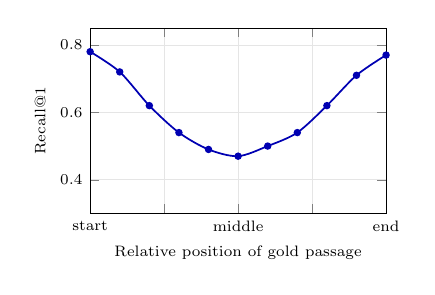
\begin{tikzpicture}[scale=0.78]
\begin{axis}[
  width=6.4cm, height=4.6cm,
  xlabel={Relative position of gold passage},
  ylabel={Recall@1},
  xmin=0, xmax=1, ymin=0.3, ymax=0.85,
  xtick={0,0.25,0.5,0.75,1.0},
  xticklabels={start,,middle,,end},
  ytick={0.4,0.6,0.8},
  grid=both,
  grid style={gray!20},
  tick label style={font=\scriptsize},
  label style={font=\scriptsize},
]
\addplot[blue!70!black, thick, smooth, mark=*, mark size=1.3pt]
  coordinates {
    (0.00, 0.78) (0.10, 0.72) (0.20, 0.62) (0.30, 0.54)
    (0.40, 0.49) (0.50, 0.47) (0.60, 0.50) (0.70, 0.54)
    (0.80, 0.62) (0.90, 0.71) (1.00, 0.77)
  };
\end{axis}
\end{tikzpicture}\\
{\scriptsize Stylized U-shape from Liu et al.\ (2024); same qualitative pattern across model families.}
\end{columns}
\end{frame}

\begin{frame}{Limit 5 --- Prompt Sensitivity and the Primacy Effect}
\begin{columns}[T]
\column{0.48\textwidth}
\textbf{Generic prompt:}
\begin{tcolorbox}[colback=blue!3, colframe=RedTitle!50, boxrule=0.3mm, arc=1mm, left=2mm, right=2mm, top=1mm, bottom=1mm]
\scriptsize\ttfamily
Classify this sentence:\\
"Inflation remains elevated and the Committee remains highly attentive to inflation risks."\\
Label:
\end{tcolorbox}
\smallskip
{\footnotesize Model output: \textit{neutral} --- the descriptive verbs (``remains'') and the absence of a directional action word dominate.}

\column{0.48\textwidth}
\textbf{Role-conditioned prompt:}
\begin{tcolorbox}[colback=green!3, colframe=green!45!black, boxrule=0.3mm, arc=1mm, left=2mm, right=2mm, top=1mm, bottom=1mm]
\scriptsize\ttfamily
You are a monetary economist. Is the following sentence hawkish, dovish, or neutral?\\
"Inflation remains elevated and the Committee remains highly attentive to inflation risks."\\
Label:
\end{tcolorbox}
\smallskip
{\footnotesize Model output: \textit{hawkish} --- ``highly attentive to inflation risks'' is read as a tightening signal once the prior is monetary policy.}
\end{columns}

\medskip
\footnotesize
\begin{itemize}\itemsep1pt
\item Both prompts pass the same sentence to the same model. The difference is the \emph{prior} the role + label space imposes (cf.\ ICL as Bayesian inference, T4).
\item \textbf{Brucks \& Toubia (2025, \emph{PLOS ONE})}: primacy bias on balanced binary tasks --- GPT-4 frequently picks the \emph{first} option (a strong, robust primacy bias). Randomize option order; average across runs.
\item \textbf{WEIRD bias} \& \textbf{version drift}: training corpus is Western/English-leaning; closed-source models change silently between API calls (T4's ``version = instrument'').
\item \textbf{Take-away.} Treat the prompt as part of the research design --- freeze it, version it, report it. Robust analyses report results under multiple paraphrases.
\end{itemize}
\end{frame}

\begin{frame}{Capstone: When the Limits Compound --- YVP (2026)}
\textbf{Three frontier models, one frozen prompt, 18{,}797 O*NET tasks --- and a 3.6$\times$ gap.}
\begin{itemize}
\item Yin, Vu \& Persico (NBER WP 35110) re-run the standard AI-exposure rubric (Eloundou et al.) with three 2025--26 frontier models --- everything else held fixed.
\item Mean exposure differs \textbf{3.6$\times$} across annotator models; pairwise agreement $\approx$57\%, Cohen's $\kappa$ as low as \textbf{0.36} (hand-coding publication standard: $\kappa \ge 0.75$).
\item Downstream, the same DiD regression on each model's scores: individual-level coefficients vary \textbf{2.4$\times$}; the county-level estimate \textbf{flips sign} (significant negative $\to$ insignificant positive).
\end{itemize}
\medskip
\begin{takeawaybox}
\textbf{Model version = measurement instrument.} Pin it, disclose it, and validate against a human gold standard --- or the regression inherits whichever model you happened to call. T5b performs the full autopsy of this literature and builds the defensive workflow.
\end{takeawaybox}
\smallskip
\textit{\footnotesize Discussion: which of the five limits drives the divergence? Mostly \#5 --- prompt/prior sensitivity compounded by each vendor's alignment choices (T4) --- with \#2 contributing at the rubric boundaries.}
\end{frame}

\begin{frame}{The Brain Metaphor}
An LLM is like a very capable brain that finished school on a fixed date.

\medskip
\begin{columns}[T]
\column{0.48\textwidth}
\begin{tcolorbox}[colback=green!5, colframe=green!40!black, title=\textbf{What the brain knows}]
\begin{itemize}
\item General language and reasoning
\item Broad economics, math, programming
\item Published papers up to its cutoff
\item Common patterns, idioms, code recipes
\end{itemize}
\end{tcolorbox}

\column{0.48\textwidth}
\begin{tcolorbox}[colback=red!5, colframe=red!50!black, title=\textbf{What the brain does \emph{not} know}]
\begin{itemize}
\item Anything that happened after the cutoff
\item Your private FOMC corpus
\item A specific firm's internal documents
\item This morning's data release
\item Your co-author's unpublished draft
\end{itemize}
\end{tcolorbox}
\end{columns}

\medskip
\textbf{Question:} how do we let this brain access the information on the right \emph{without} retraining it? (Lecture 8's opening question --- and T5b's closing bridge.)
\end{frame}

%=============================================================================
\begin{frame}{Bridge: Knowing the Limits, Use the Strengths}
\textbf{The audit is done; now the toolkit.}
\begin{itemize}
\item Nothing in this deck says ``don't use LLMs.'' It says \emph{unvalidated} use is what fails --- and each limit has a research-design counter: ground it, pin it, audit it, randomize it.
\item \textbf{T5b:} what embeddings already measure (similarity, classification, networks); the case-study record from ECB Word2Prices to asset embeddings; the AI-exposure cautionary tale in full; and the six-step validation workflow --- ending on the lecture's thesis.
\end{itemize}
\bigskip
\centering\footnotesize\textit{Arc: T1 FRAME $\to$ T2 REPRESENT $\to$ T3 ATTEND $\to$ T4 PRETRAIN $\to$ \textbf{T5 MEASURE}.}
\end{frame}

\end{document}
